   Cette strat\'egie de test, comme toute strat\'egie de test, cherche \`a remplir trois objectifs :
   
\begin{itemize}
       
\item am\'eliorer la productivit\'e du d\'eveloppement d'applications
     distribu\'ees \`a interface l\'eg\`eres (ie. des applications J2EE et
     \'eventuellement .Net) en permettant d'identifier et donc de
     corriger le plus t\^ot possible les erreurs de d\'eveloppement, les
     incoh\'erences entre la conception et le d\'eveloppement, voire
     am\'eliorer la conception pour permettre la testabilit\'e des
     artefacts produit lors de cette phase essentielle ; 
\item am\'eliorer la qualit\'e du logiciel r\'esultant afin de r\'eduire les
     co\^uts de maintenance et d'accro\^{\i}tre la satisfaction des
     utilisateurs ; 
\item permetter de d\'egager du temps de d\'eveloppement
     
\emph{stupide}
   pour effectuer des t\^aches plus int\'eressantes
     de conception, d'architecture et de v\'erification.
\end{itemize}
  
   Pour atteindre cet objectif, j'estime qu'il est n\'ecessaire de
   maximiser l'
\emph{automatisation}
   de toutes les phases du
   processus de d\'eveloppement qui le permette, et en particulier les
   phases de r\'ealisation, d'ex\'ecution et de rapport des tests. 
  
\par
  
   Ce document est inspir\'ee en grande partie par les diverses exp\'eriences v\'ecues
   de d\'eveloppement au sein de Norsys sur des projets J2EE, mes
   lectures  et plus particuli\`erement le livre de Robert
   Binder sur le test orient\'e objet et mes travaux de recherche. 
   On notera par ailleurs que les tests ne sont qu'un \'el\'ement
   d'une strat\'egie globale de contr\^ole de la qualit\'e d'une
   application et doit s'accompagner d'un certains nombre d'autres
   proc\'edures de v\'erification telles que la revue de code, les
   analyses statiques du code et/ou du bytecode, la v\'erification du
   respect de l'architecture, la preuve ...
  
\par
  
\section{Processus}
  
\subsection{Echelle de test}
  
    Le test peut-\^etre conduit \`a diff\'erents niveaux de
    granularit\'es. Dans chaque cas, le test est r\'ealis\'e par ex\'ecution
    de tests sur l'interface (au sens le plus large) de l'objet test\'e en fonction des
    exigences op\'erationnelles d\'efinies pour cet objet. Pour les
    besoins des applications J2EE, on identifie 5 niveaux  :
    
\begin{enumerate}
       
\item 
\textbf{classes :}
   la classe est la plus petite entit\'e
     testable du processus de d\'eveloppement. Bien que l'on puisse
     envisager de d\'evelopper des tests sp\'ecifiques au niveau des
     m\'ethodes, la classe est l'unit\'e de d\'eveloppement logique de toute
     application objet, c'est une unit\'e d'encapsulation et
     d'ex\'ecution. Dans un certain nombre de cas, il est m\^eme difficile
     d'envisager de tester chaque classe isol\'ement, on parlera alors
     de 
\emph{clusters}
   de classes lorsque le couplage est
     fort. Par exemple, il est difficile de tester une classe
     
\texttt{Graphe}
   sans tester les classes 
\texttt{Noeud}
   et
     
\texttt{Arc}
  . Dans le cas de hi\'erarchies de classes (hors les
     cas des frameworks), les classes de bases et sous-classes sont
     consid\'er\'ees soient globalement lorsqu'elles sont toutes connues,
     soit de haut en bas lorsqu'elles sont d\'evelopp\'ees
     ind\'ependamment. Les tests pour une sous-classes inclus
     normalement les tests pour la super-classe.  ; 
\item 
\textbf{composants :}
   un composant est un ensemble de classes
     r\'ealisant une fonctionnalit\'e pr\'ecise et accessible au travers
     d'une ou plusieurs interfaces (au sens Java). Une couche d'une application
     multicouche est un composant. Un composant est test\'e en isolement
     par simulation de son environnement (cf. r\'ealisation de Mock
     Objects) ;  
\item 
\textbf{frameworks : }
   un framework est un composant
     r\'eutilisable par h\'eritage et aggr\'egation. Une classe g\'en\'erique
     est un framework r\'eduit \`a une seule classe. Un framework est
     compos\'e de classes et \'eventuellement de composants internes. Un framework
     ne peut \^etre test\'e sans instantiation d'une partie des classes
     abstraites qu'il expose. L'interface d'un framework  
\item 
\textbf{sous-syst\`eme :}
   un sous-syst\`eme est un ensemble de
     classes, composants et frameworks r\'ealisant une partie des
     fonctionnalit\'es du syst\`eme global et ex\'ecutable
     isolement. Typiquement, un sous-syst\`eme sera identifi\'e \`a un
     ensemble de fonctionnalit\'es de l'application et donc \`a un
     ensemble de cas d'utilisation. Le test d'un sous-syst\`eme est
     r\'ealis\'e soit  sur un environnement proche de l'environnement
     final, soit confin\'e dans un environnement simul\'e  
\item 
\textbf{syst\`eme : }
   un syst\`eme est l'objectif de r\'ealisation
     du processus de d\'eveloppement, constitu\'e d'\'el\'ements \`a diff\'erents
     niveaux de granularit\'es. Le test du syst\`eme est r\'ealis\'e dans
     l'environnement le plus proche possible de l'environnement de
     production. Les tests \`a l'\'echelle du syst\`eme incluent les tests
     de performances, d'int\'egrit\'e et de tol\'erance aux pannes, d'IHM,
     de configuration et de compatibilit\'e, en sus bien \'evidemment de
     l'ensemble des tests dit fonctionnels. On parlera de pr\'ef\'erence
     des exigences sur le syst\`eme pour englober toutes les contraintes
     auxquelles doient r\'epondre celui-ci et les besoins qu'il doit
     satisfaire. Les tests post\'erieurs \`a la phase de d\'eveloppement :
     alpha-tests, beta-tests, tests de recette et tests de conformit\'e
     (au sens de conformit\'e aux normes) ne rentrent pas dans la port\'ee
     de ce document.
\end{enumerate}
  
\par
  
\subsection{Granularit\'e}
  
    La notion de 
\emph{test unitaire}
   est g\'en\'eralement entendue
    en son sens le plus \'etroit de "test d'une unit\'e de
    d\'eveloppement". On pr\'ef\'erera distinguer deux types de tests
    compl\'ementaires, applicables \`a tous les niveaux d'\'echelle :
    
\begin{itemize}
       
\item d'une part les tests fonctionnels, c'est-\`a-dire les test
      bas\'es sur les fonctionnalit\'es attendues de l'objet test\'e et qui
      visent \`a valider la conformit\'e du comportement de l'objet avec
      ses sp\'ecifications (quelles que soient les formes que prennent
      celles-ci). L'objectif du test fonctionnel et de maximiser un
       crit\`ere de couverture d\'ependant de l'objet test\'e : couverture du
      code de la classe ou du cluster, couverture des chemins d'un
      graphe de contr\^ole d\'eduit d'un diagramme de s\'equence, ...
      
\item 
       d'autre part les tests d'int\'egration, qui visent \`a v\'erifier que
      la composition d'objets de niveau N pour produire un objet de
      niveau N+1 fonctionne 
\emph{a minima}
  . L'objectif du test
      d'int\'egration est d'assurer l'interop\'erabilit\'e des objets en
      maximisant la couverture des interactions possibles entre les
      objets : appels de m\'ethodes, transferts de donn\'ees, ...
     
\end{itemize}
  
\par
  
\par
  
\subsection{Mod\`ele g\'en\'eral d'un processus de test}
  Le processus de v\'erification d'un logiciel en construction \`a
    l'aide de tests est identique, quelle que soit l'\'echelle
    consid\'er\'ee. 
    
\begin{enumerate}
       
\item on dispose d'un objet \`a tester ou CUT - 
\emph{Component Under
      Test}
   -  \'eventuellement compos\'e
      d'objets de plus petite \'echelle suppos\'es d\'ej\`a test\'es ; 
\item la premi\`ere \'etape du test est  le 
\emph{test
      d'int\'egration}
   qui s'assure de l'interop\'erabilit\'e des
      objets test\'es et v\'erifie que les tests pourront bien \^etre
      ex\'ecut\'es sur le CUT ; 
\item on d\'eveloppe une suite de test \`a partir des sp\'ecifications
      du CUT, c'est \`a dire en fonction de ses responsabilit\'es ; 
\item \'eventuellement, on d\'eveloppe et on installe
      l'infrastructure de test n\'ecessaire au CUT, en particulier les
      drivers et les bouchons ; 
\item la suite de tests est ex\'ecut\'ee
      
\begin{enumerate}
       
\item si certains tests \'echouent, on retourne le CUT en phase de
      d\'eveloppement pour correction des erreurs, 
\item sinon, on passe \`a l'\'etape suivante ;
\end{enumerate}
   
\item on compare la couverture r\'ealis\'ee par la suite de test avec
      l'objectif de couverture pr\'ealablement d\'efini :
      
\begin{enumerate}
       
\item si l'objectif est atteint, le CUT est consid\'er\'e test\'e et
      l'on peut passer \`a une autre phase de test, 
\item sinon, on retourne \`a la phase de conception de la suite
      de test pour l'augmenter. On peut \^etre amen\'e dans cette phase \`a
      examiner l'implantation du composant test\'e pour atteindre
      l'objectif de couverture  en d\'efinissant des cas de tests non
      pr\'evus par les sp\'ecifications mais r\'ealisables dans le
      code. C'est aussi \`a cette phase que l'on peut identifier des
      probl\`emes de coh\'erences entre code et sp\'ecification : code mort,
      surprises, sp\'ecifications incompl\`etes,
      ...
\end{enumerate}
  
\end{enumerate}
  
Ce processus est synth\'etis\'e dans la figure 
\ref{fig-process-test}
  . Il est d\'eclinable \`a diff\'erentes
      \'echelles en param\'etrant correctement l'ensemble des phases en
      fonction des objets manipul\'es : classes unitaires, cluster de
      classes, composant, sous-syst\`eme, syst\`eme.
\par
  
\begin{figure}
\centering
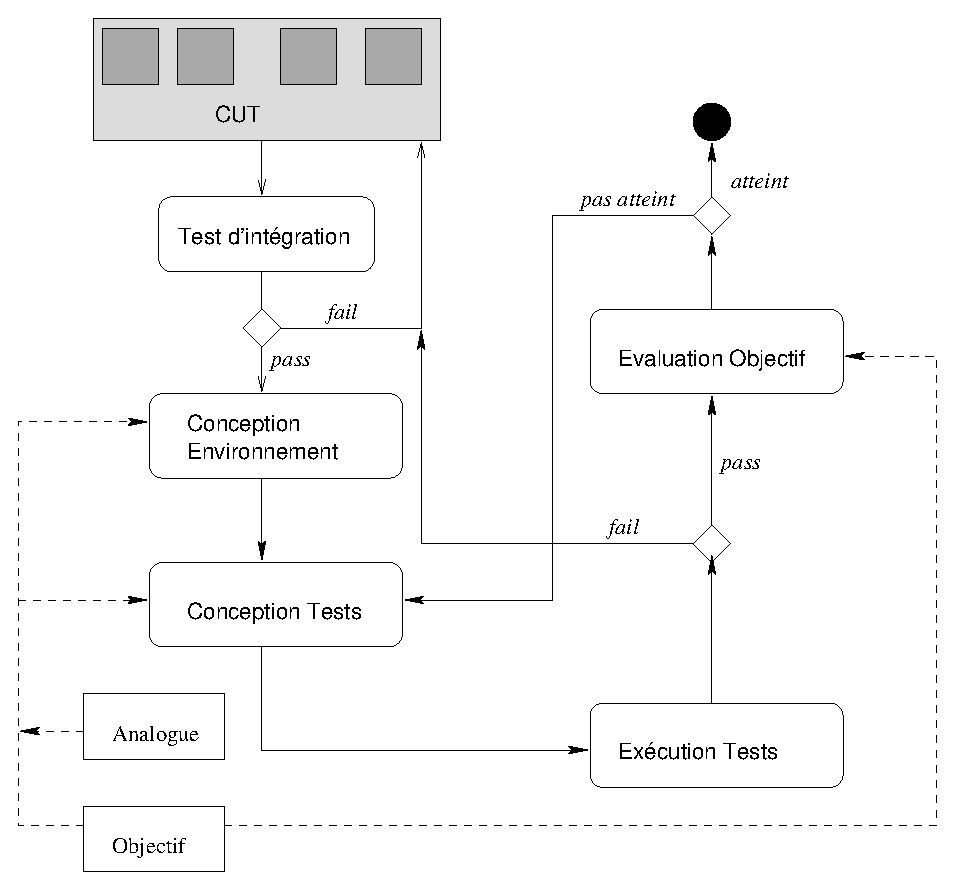
\includegraphics{figures/fig-processtest.eps}
\caption{Interaction    fonctionnel/int\'egration}
\label{fig-process-test}
\end{figure}
 
\subsection{Phases de d\'eveloppement}
  
    Tous les tests ne sont pas con\c{c}us d\`es la conception du
    projet ni jou\'es une seule fois \`a la fin du projet, les
    processus de tests \`a diff\'erentes \'echelles s'int\`egrent
    dans le processus global de d\'eveloppement du logiciel. 
    
\par
  A notre avis, les tests font partie des \'el\'ements de
   v\'erification dynamiques et statiques permettant de franchir des
   transitions dans le d\'eveloppement du logiciel : prototypage du
   produit, ajout de nouvelles fonctionnalit\'es, mise en recettage
   et mise en production, maintenance, \'evolutions fonctionnelles,
   ...
   
\par
  
    On va donc d\'efinir une hi\'erarchie des tests, \`a
    diff\'erents niveaux de granularit\'e, dans l'objectif de
    constituer une suite de test globale \`a l'application. Pour
    chaque \'el\'ement de cette hi\'erarchie, on indique :
    
\begin{itemize}
       
\item l'objectif g\'en\'eral du test ; 
\item le mod\`ele de fautes que l'on cherche \`a identifier par
     les tests ; 
\item le ou les objets sur lesquels portent les test ; 
\item le mod\`ele depuis lequel sont d\'eriv\'es les cas de
     test ; 
\item les crit\`eres d'op\'erabilit\'e minimaux pour
     l'ex\'ecution des tests de la hi\'erarchie (tests
     d'int\'egration) ; 
\item l'interface par laquelle les tests vont exercer le
     fonctionnement de l'objet \`a tester ; 
\item les objectifs de couverture \`a atteindre pour valider les
     tests de cette hi\'erarchie ; 
\item la proc\'edure de d\'erivation des cas de tests ; 
\item l'environnement de test n\'ecessaire \`a l'ex\'ecution
     des tests de cette hi\'erarchie ; 
\item la proc\'edure d'ex\'ecution des cas de tests.
\end{itemize}
  
\par
  
\subsubsection{Tests de classes}
  
\textbf{Objectif :}
  s'assurer que la classe ou le cluster de
    classes respecte le contrat d\'efini soit directement par la
    sp\'ecification de la classe, soit indirectement par les
    sp\'ecifications de ses super-classes.
\par
  
\textbf{Fautes :}
  
\par
  
\textbf{Objets :}
   le CUT est une instance de la classe ou du
    cluster de classe consid\'er\'e.
\par
  
\textbf{Mod\`ele :}
   le mod\`ele utilis\'e est la description
    des fonctionnalit\'es attendues de la classe et \'eventuellement
    celle de la
    hi\'erarchie dont elle fait partie. Ce mod\`ele peut prendre
    diff\'erentes formes : description textuelles, invariants et
    pre/post conditions, automate, ou une combinaison de ces \'el\'ements.

\par
  
\textbf{Op\'erabilit\'e : }
  la ou les classes
    consid\'er\'ees doivent bien \'evidemment \^etre compil\'ees
    sans erreur. La classe doit \^etre 
\emph{observable}
  , c'est
    \`a dire que son \'etat interne doit pouvoir \^etre observ\'e
    sans ambig\"uit\'e \`a l'aide des m\'ethodes 
\texttt{get}
  
    appropri\'eess ; elle doit \^etre 
\emph{contr\^olable}
  ,
    c'est \`a dire que son comportement doit d\'ependre uniquement
    des m\'ethodes publiques qu'elle d\'efinit, directement ou
    indirectement (par l'interm\'ediaire de sa hi\'erarchie de
    classe). 
\par
  
\textbf{Interface :}
  la classe va \^etre test\'ee au moyen de
    ses m\'ethodes publiques, d\'efinies ou h\'erit\'ees.
\par
  
\textbf{Couverture : }
  les objectifs de couverture peuvent
    \^etre vari\'ees suivant le degr\'e de confiance
    n\'ecessaire. Une \'evaluation des risques pr\'ealables permet
    de positionner le curseur de mani\`ere ad\'equate : une classe
    de type value-object n'a pas les m\^emes besoins de couverture
    qu'une classe contr\^oleur ou une classe fondation sur laquelle
    vont s'appuyer un ensemble de classes. L'analyse du graphe de
    d\'ependance permet d'identifier les classes les plus
    utilis\'ees. La couverture du test de classes doit prendre en
    compte non seulement le flot d'ex\'ecution des m\'ethodes
    individuelles, mais aussi les d\'ependances existant entre
    m\'ethodes, notamment les d\'ependances  li\'ees \`a la
    d\'efinition et l'utilisation des attributs de la classe et de la
    super-classe. La couverture est atteindre peut-\^etre, par ordre
    croissant de fiabilit\'e (et d'effort de test) :
     
\begin{itemize}
       
\item couverture des m\'ethodes : toutes les m\'ethodes
      ont \'et\'e ex\'ecut\'ees au moins une fois ; 
\item couverture des instructions : toutes les
      instructions/expressions ont \'et\'e ex\'ecut\'ees au moins
      une fois ; 
\item couverture des branches : toutes les branches ont
      \'et\'e ex\'ecut\'ees au moins une fois ; 
\item couverture des conditions : toutes les combinaisons
      possibles d'expression conditionnelles compos\'ees modifiant le
      chemin d'ex\'ecution ont \'et\'e ex\'ecut\'ees ; 
\item couverture des boucles \`a profondeur N : toutes les
      boucles ont \'et\'e ex\'ecut\'ees au moins N fois  ; 
\item couverture alpha-omega : tous les chemins d'ex\'ecution
      entre la cr\'eation de l'objet et sa destruction ont \'et\'e
       ex\'ecut\'es ; 
\item couverture des DU-chemins : tous
      les chemins menant d'une d\'efinition d'une variable \`a une
      utilisation d'une variable ont \'et\'e test\'ees. Les
      variables contiennent aussi les attributs de l'objet
      consid\'er\'e et ceux de tous les objets qu'il  manipule ou
      dont il h\'erite : l'appel \`a un constructeur ou un mutateur
      est une d\'efinition de variable, m\^eme si techniquement la
      variable r\'ef\'erencant l'objet ne change pas ; 
\item ... 
\item couverture exhaustive : impraticable mais offre un niveau
      de confiance maximal !
\end{itemize}
  
\par
  
\textbf{D\'erivation des cas de tests :}
   la suite de test
      initiale est d\'eriv\'ee par application des techniques
      standards de partitionnement des variables, de parcours du
      graphe mod\'elisant le comportement de la classe, de
      l'analyse des fonctionnalit\'es attendues de la classe, de
      l'intuition du testeur sur les responsabilit\'es de la
      classe. Cette suite de tests doit \^etre enrichie tant que le
      crit\`ere de couverture n'est pas atteint par analyse du code
      des objets. La suite de tests prend la forme d'une ou plusieurs
      classes 
\texttt{TestCase}
    ;
\par
  
\textbf{Environnement :}
  les d\'ependances du CUT doivent
      \^etre remplac\'ees en tant que de besoin par des Mock Objects
      dont le comportement est controll\'e par l'environnement en
      fonction des sp\'ecifications de ces classes. Ces Mock Objects
      peuvent \^etre d\'eriv\'ees automatiquement, en utilisant un
      outil ad\'equat, ou manuellement par le testeur.

\par
  
\textbf{Ex\'ecution :}
   les tests sont ex\'ecut\'ees dans
      l'environnement de d\'eveloppement par invocation de JUnit, ou
      lors de la construction it\'erative de l'application.
\par
  
\subsubsection{Tests de composants}
  
    Par composant, on entend aussi bien des composants de service que
    des composants fonctionnels. Dans le cas d'application orient\'e
    Web bas\'ees sur Struts ou \'equivalent, un composant sera
    d\'efini comme un ou plusieurs \'el\'ements r\'ealisant une
    fonctionnalit\'e de l'application : action Struts, JSP, forms,
    ... Dans les cas de composants m\'etier  EJB, le composant sera
    g\'en\'eralement limit\'e \`a l'EJB lui-m\^eme et \`a ses
    interfaces 
\texttt{Remote}
   et 
\texttt{Home}
  , plus
    \'eventuellement les classes sp\'ecifiques \`a cet EJB
    utilis\'ees dans son contexte.
    
\textbf{Objectif :}
   s'assurer que la ou les interfaces du composant test\'e
    r\'epondent \`a leurs sp\'ecifications.
\par
  
\textbf{Fautes :}
   configuration du composant incompl\`ete ou
    mal g\'er\'ee, probl\`eme de polymorphisme des m\'ethodes,
    probl\`emes li\'es \`a l'ex\'ecution concurrente, ...
\par
  
\textbf{Objets :}
   le CUT est une instance du composant test\'e.
\par
  
\textbf{Mod\`ele :}
   le mod\`ele utilis\'e est la description
    des fonctionnalit\'es attendues du composant. Ce mod\`ele peut prendre
    diff\'erentes formes : description textuelles, invariants et
    pre/post conditions sur les interfaces, automate, cas
    d'utilisation avec diagrammes de s\'equences d\'ecrivant
    l'utilisation du composant, ...

\par
  
\textbf{Op\'erabilit\'e : }
  les classes dont est compos\'e le
    CUT doivent avoir pass\'e les 
\emph{tests de niveau
    classe}
  . Les tests d'int\'egration relatifs
    \`a la composition de ces objets doivent avoir \'et\'e
    ex\'ecut\'ees par aggr\'egation succesive des objets selon
    leurs d\'ependances (cf. infra). L'\'etat interne du composant
    doit pouvoir \^etre observ\'e, soit au travers des m\'ethodes
    des intefaces, soit par instrumentation du composant
    (cf. Observation intrusive), soit par positionnement des
    assertions (pour les versions de la plateforme les supportant, en
    l'occurence pour Java \`a partir du JDK 1.4).
\par
  
\textbf{Interface :}
   le composant est test\'e au travers de
    toutes ses interfaces publiques, y compris les m\'ethodes factory
    propos\'ees.
\par
  
\textbf{Couverture : }
   les objectifs de couverture peuvent
    \^etre soit fonction de la sp\'ecification du composant, soit
    similaires aux objectifs de couverture pour les classes restreints
    aux interfaces du composant et \`a ses d\'ependances. Dans le
    premier cas, on cherchera \`a disposer d'un mod\`ele sous forme
    d'automate ou de graphe de contr\^ole de l'\'etat du
    composant sur lequel on applique les crit\`eres de couverture
    d\'efinis ci-dessus. 
\par
  
\textbf{D\'erivation des cas de tests :}
   identique au niveau classe.
\par
  
\textbf{Environnement :}
   identique au niveau classe.

\par
  
\textbf{Ex\'ecution :}
   ibidem.
\par
  
\subsubsection{Tests de frameworks}
  
    Les tests de framework sont d\'efinis par le producteur du
    framework mais utilis\'es par le consommateur. Il s'agit d'une
    
\emph{suite de conformit\'e}
   permettant au d\'eveloppeur
    utilisant le framework de s'assurer de sa bonne utilisation.
    Dans le cas du test d'un framework en cours de d\'eveloppement,
    une implantation de r\'ef\'erence assurera l'op\'erabilit\'e
    du framework et permettra de produire la suite de conformit\'e
    fournie avec le framework.
    
\textbf{Objectif :}
   s'assurer de la conformit\'e d'une
    utilisation - implantation - concr\`ete du framework.
\par
  
\textbf{Fautes :}
   toutes les erreurs dans l'utilisation du
    framework, en particulier : non respect des contrats d'interfaces
    ou de classes abstraites implant\'ees, mauvaise utilisation des
    m\'ethodes, mauvaise s\'equence d'appels de m\'ethodes, erreurs
    de configuration, ...
\par
  
\textbf{Objets :}
   le CUT est constitu\'e du framework, de son
    instance et des \'el\'ements de configuration n\'ecessaires,
    \'eventuellement adapt\'es \`a l'environnement de test
    (properties, variables d'environnement, variables globales,
    param\`etres d'extension Java, ...) 
\par
  
\textbf{Mod\`ele :}
   comme pour le test de composant. On
    utilisera un mod\`ele des fonctionnalit\'es du framework et des
    contrats sur ses instances : cas d'utilisation et diagrammes de
    s\'equences, automates, ...
\par
  
\textbf{Op\'erabilit\'e : }
   les classes participant au
    framework doivent avoir pass\'e les tests de niveau classe. Les
    tests d'int\'egration pour les diff\'erents composants du
    framework et de l'instance consid\'er\'e doivent avoir \'et\'e
    ex\'ecut\'ees. 
\par
  
\textbf{Couverture :  }
   l'objectif de couverture est d\'efini
    \`a la fois par les sp\'ecifications du framework et par la
    couverture des classes participantes de l'instanciation. En
    particulier, cet objectif doit prendre en compte les cas
    d'utilisation d\'efinis par le mod\`ele du framework, les
    associations entre classes du framework et classes instanci\'ees
    et \'eventuellement l'automate de contr\^ole d\'ecrivant le
    comportement du framework.
\par
  
\textbf{D\'erivation des cas de tests :}
  comme pour le niveau
    classe. 
\par
  
\textbf{Environnement :}
   selon les cas, soit un environnement
    simul\'e, soit un environnement r\'eel de test proche de la
    cible de d\'eploiement finale.
\par
  
\subsubsection{Test de sous-syst\`emes}
  
\textbf{Objectif :}
  
\par
  
\textbf{Fautes :}
  
\par
  
\textbf{Objets :}
  
\par
  
\textbf{Mod\`ele :}
  
\par
  
\textbf{Op\'erabilit\'e : }
  
\par
  
\textbf{Couverture :  }
  
\par
  
\textbf{D\'erivation des cas de tests :}
  
\par
  
\textbf{Environnement :}
  
\par
  
\subsubsection{Test de syst\`emes}
  
\textbf{Objectif :}
  
\par
  
\textbf{Fautes :}
  
\par
  
\textbf{Objets :}
  
\par
  
\textbf{Mod\`ele :}
  
\par
  
\textbf{Op\'erabilit\'e : }
  
\par
  
\textbf{Couverture :  }
  
\par
  
\textbf{D\'erivation des cas de tests :}
  
\par
  
\textbf{Environnement :}
  
\par
  
\subsubsection{Test d'int\'egration}
  
    Nous consid\'erons ici un sch\'ema de test d'int\'egration
   g\'en\'erique applicable \`a diff\'erents niveaux de la
   hi\'erarchie de test. Les cas particuliers d'int\'egration
   relatifs aux diff\'erents niveaux sont d\'ecrits ci-dessus dans
   les sch\'emas de test. 
   
\textbf{Objectif :}
   s'assurer de l'interop\'erabilit\'e des
   diff\'erents composants aggreg\'es par un CUT. La phase de test
   d'int\'egration est un pr\'ealable \`a l'ex\'ecution des tests
   unitaires. 
\par
  
\textbf{Fautes :}
   on cherche a r\'ev\'eler des fautes
   relatives \`a l'interaction des diff\'erents objets : erreurs
   dans les versions (g\'en\'eralement d\'etect\'ees \`a la
   compilation mais pas toujours, surtout dans les cas de chargement
   dynamique de classes), utilisation incorrecte des contrats d'objets
   (param\`etres incorrects, par exemple valeurs nulles, non respect
   des pr\'e-conditions), erreurs dans les associations entre
   classes, erreurs dans l'acc\`es aux ressources, erreurs dans
   l'allocation de ressources, ... Dans la mesure o\`u l'on suppose
   que les diff\'erentes parties de l'interaction ont \'et\'e
   test\'ees isol\`ement, les erreurs proviennent essentiellement du
   non-respect ou de la mauvaise interpr\'etation par des clients (au
   sens d'objets utilisateur de services) des contrats d'un serveur
   (au sens d'objet fournisseur de services).
\par
  
\textbf{Objets :}
   les diff\'erents parties composant le CUT et
   le CUT lui-m\^eme avec les ressources n\'ecessaires \`a son fonctionnement.
\par
  
\textbf{Mod\`ele :}
   mod\`ele des d\'ependances ou
   interactions entre composants : cas d'utilisation avec s\'equences ou collaborations,
   graphe de d\'ependances. 
\par
  
\textbf{Op\'erabilit\'e : }
   les diff\'erentes parties \`a
   int\'egrer doivent avoir pass\'e leurs tests unitaires.
\par
  
\textbf{Couverture : }
   l'objectif de couverture est d\'efini en
   fonction des d\'ependances entre les parties \`a int\'egrer. La
   couverture minimale \`a atteindre est de couvrir par
   l'ex\'ecution au  moins chaque paire de m\'ethodes
   appelantes-appel\'ees, m\'ethodes pouvant s'entendre  ici au sens
   plus g\'en\'eral de code g\'en\'erant une requ\^ete et de code
   r\'epondant \`a une requ\^ete.
\par
  
\textbf{D\'erivation des cas de tests :}
   les cas de tests sont
   d\'eriv\'es de telle sorte \`a exercer les liens existant entre
   composants. Binder pr\'esente diverses strat\'egies
   d'int\'egration qui permettent de g\'en\'erer diff\'erents
   ensembles de suites de test : 
     
\begin{itemize}
       
\item Big-bang : toutes les parties sont test\'ees
   simultan\'ement; 
\item Top-down : les parties sont  int\'egr\'ees succesivement
   depuis l'\'el\'ement le plus d\'ependant, g\'en\'eralement
   l'interface du CUT, vers les \'el\'ements de plus bas niveau. Le
   m\^eme driver de test est utilis\'e pour tous les tests et des
   Mock Objects sont g\'en\'er\'es en fonction des besoins ; 
\item Bottom-up : les parties sont int\'egr\'ees depuis les
   couches les plus basses vers les couches les plus hautes en
   d\'eveloppant des drivers sp\'ecifiques \`a chaque \'etape et
   en int\'egrant les \'el\'ements d\'ej\`a test\'es ; 
\item Collaboration : les parties sont test\'ees en fonction de
   leur participation \`a diff\'erentes collaborations :
   sc\'enarios, use-cases, s\'equences, ... Les collaborations
   test\'ees sont ensuite int\'egr\'ees globalement ; 
\item Couche : les diff\'erentes parties sont int\'egr\'ees
   couches par couches, soit bottom-up, soit top-down.
\end{itemize}
  
\par
  
\textbf{Environnement :}
   selon les cas, l'int\'egration est
   test\'ee dans un environnement simul\'e ou dans l'environnement
   cible. 
\par
  
\section{Mod\`eles}
  
   Un mod\`ele de test est une sp\'ecification testable de l'objet sous
   test, c'est-\`a-dire une sp\'ecification \`a partir de laquelle on peut
   d\'eriver des tests. Il en existe de tr\`es nombreux mais grosso modo
   on se ram\`ene syst\'ematiquement \`a deux formes de mod\`eles :
   
\begin{itemize}
       
\item des mod\`eles d\'ecrivant le comportement \`a tester de l'objet
    sous la forme d'un automate d'\'etats finis ; 
\item des mod\`eles combinatoires d\'ecrivant l'objet \`a tester sous la
    forme d'une relation entre des pr\'edicats sur des valeurs d'entr\'ee
    et des valeurs de sorties (valeur de retour, \'etat du syst\`eme,
    actions r\'ealis\'ees, ...) ;
\end{itemize}
  
\par
  
\subsection{Automates}
  
    Par 
\emph{automates}
   nous entendons tous les mod\`eles se
    pr\'esentant sous la forme de diagrammes d'\'etats/transitions :
    statecharts, graphe de contr\^ole, machines d'\'etats finis, c'est \`a
    dire tout mod\`ele dans lequel les \'etats de l'objet et les
    transitions permettant de passer d'un \'etat \`a un autre sont
    mod\'elis\'ees. De tr\`es nombreux mod\`eles de plus haut niveau, en
    particulier les diagrammes UML d'activit\'e, de collaboration, de
    s\'equence, voire des descriptions textuelles de sc\'enario, sont
    traduisibles en termes d'automates. Nous nous contenterons ici de
    mod\`eles d'automates simples : un \'etat d'entr\'ee, $n$
    \'etats de sortie, ensemble d'\'etats et de transitions finies.
    
\par
  Le principal int\'er\^et de ce type de mod\`ele est qu'il se pr\^ete
    particuli\`erement bien \`a la construction de suites de test en
    offrant \`a la fois une sp\'ecification et si besoin une mesure de la
    couverture de l'effort de  test. Il existe une vaste litt\'erature
    th\'eorique consacr\'ee au test d'automates - et mod\`eles similaires -
    avec un grand nombre d'algorithme permettant de s'assurer de
    certaines propri\'et\'es du CUT sous r\'eserve d'hypoth\`eses
    simplificatrice sur son implantation.
\par
  
    Le principe g\'en\'eral de la g\'en\'eration de suites de
    tests \`a partir d'automates est simple :
    
\begin{itemize}
       
\item choisir l'\'etat cible que l'on souhaite tester ; 
\item d\'efinir un 
\texttt{pr\'eambule}
   sens\'e
      positionner le CUT dans l'\'etat choisi. Ce pr\'eambule est un
      chemin dans l'automate connect\'e \`a l'\'etat
      s\'electionn\'e. Selon les cas, il peut \^etre n\'ecessaire
      de positionner des objets dans un \'etat sp\'ecifique, choisir
      des valeurs de variable, d'attributs ou de param\`etres pour une
      ou plusieurs m\'ethodes, positionner des variables globales,
      ... 
\item s\'electionner une transition \`a tester depuis l'\'etat
      choisi et d\'efinir les variables d'entr\'ee n\'ecessaire
      pour franchir cette transition ; 
\item d\'efinir un 
\emph{oracle}
   permettant de v\'erifier que
      l'\'etat atteint lors du franchissement de la transition est le
      bon : selon les cas, il peut s'agir de v\'erifier l'\'etat de
      l'objet, une ou plusieurs valeurs de retour, des messages \'emis
      (appels de m\'ethodes, requ\^etes, ...), de la modification de
      variables globales ou d'autres ressources ; 
\item ex\'ecuter la s\'equence de test d\'efinie ci-dessus
     ; 
\item appliquer l'oracle et comparer le r\'esultat \`a l'\'etat pr\'evu
     dans le mod\`ele.
\end{itemize}
  
\par
  
\subsubsection{Contraintes}
  Pour qu'un mod\`ele sous forme d'automate soit utilisable,
    c'est \`a dire testable, il est n\'ecessaire de respecter un certain
    nombre de contraintes et de faire des hypoth\`eses sur
     l'implantation. 
     
\begin{itemize}
       
\item les \'etats doivent \^etre 
\emph{observables}
  , c'est \`a
      dire que l'on doit pouvoir savoir dans quel \'etat pr\'ecis se
      trouve le CUT ; 
\item l'automate mod\`elisant le CUT doit \^etre
      
\emph{d\'eterministe}
   - il n'existe pas deux transitions
      identiques menant dans deux \'etats diff\'erents \`a partir d'un m\^eme
      \'etat, 
\emph{complet}
   - tous les couples \'etats-transitions
      doivent \^etre pr\'esents dans le mod\`ele, au besoin en pr\'ecisant une
      ou plusieurs actions par d\'efauts (par exemple la lev\'ee
      d'exceptions), et 
\emph{fortement connexe}
   tous les \'etats
      doivent \^etre accessibles depuis n'importe quel autre \'etat (sauf
      l'\'etat initial et un \'eventuel \'etat final unique) ; 
\item le CUT doit \^etre controllable, c'est \`a dire que l'on doit
      pouvoir le positionner dans un \'etat particulier au moyen de son
      interface.
\end{itemize}
  
\par
  
\subsubsection{Crit\`eres de couverture}
  
    La g\'en\'eration de tests \`a partir d'automates utilise g\'en\'eralement
    le mod\`ele lui-m\^eme pour d\'efinir un crit\`ere de
    couverture. Diff\'erents crit\`eres existent hi\'erarchiquement reli\'es, comme pour la couverture
    de code : couverture des \'etats, couverture de toutes les
    transitions, couverture de toutes les s\'equences de longueur N,
    couverture de tous les chemins alpha-om\'egas, couverture de tous
    les chemins (impraticables en g\'en\'eral).
\par
  Binder propose une m\'ethode de g\'en\'eration de cas de tests,
    appel\'ee N+ pour le mod\`ele FREE. Cette couverture revient \`a une
    couverture de toutes les transitions pour un mod\`ele incompl\`etement
    sp\'ecifi\'e. Elle permet de d\'etecter toutes les erreurs de sortie,
    c'est \`a dire toutes les transitions produisant une action
    incorrecte, et la plupart des  erreurs de transfert (transitions
    omises ou ajout\'ees). Elle suppose toutefois une confiance dans
    l'observation de l'\'etat du CUT.
\par
  Des crit\`eres plus puissants existent lorsque l'\'etat du CUT
    n'est pas observable directement : il est n\'ecessaire de le d\'eduire
    des actions produites et la v\'erification des erreurs impliquent de
    produire des s\'equences de test permettant de v\'erifier cette
    
\emph{signature}
  . Si l'on suppose en plus l'existence
    d'\'etats non sp\'ecifi\'es, il devient n\'ecessaire de construire des
    s\'equences encore plus longues (cf. document sur le test de FSM).
\par
  
\subsubsection{Sp\'ecificit\'es de l'objet}
  La principale difficult\'e li\'ee au test de logiciels objets
    \`a partir d'automates se situe dans l'h\'eritage. La plupart
    des m\'ethodes de conception OO proposent une forme ou une autre
    d'automates hi\'erarchiques, inspir\'es des Statecharts de Harel,
    permettant entre autre de mod\'eliser ces particularit\'es au travers
    d'\'etats orthogonaux - extension de comportement - et d'\'etats
    imbriqu\'es - sp\'ecialisation du comportement. Il est
    clair toutefois que  si l'on souhaite maintenir une relation de
    sous-typage forte, c'est \`a dire respectant le principe de
    substitution de Liskov - le comportement d'une sous-classe est
    indistinguable de celui d'une super-classe si celle-l\`a est utilis\'ee au
    travers de l'interface de celle-ci - il est n\'ecessaire d'imposer
    un certain nombres de limites, en particulier : tous les \'etats et
    toutes les transitions  d'une super-classe doivent \^etre pr\'esents
    dans le mod\`ele de la sous-classe.
    
\par
  
    La notion d'automate hi\'erarchique est toutefois une simple
    facilit\'e syntaxique offerte aux concepteurs : pour \^etre testable,
    ces mod\`eles doivent \^etre aplatis, ce qui correspond d'ailleurs \`a
    la s\'emantique usuelle des Statecharts d\'efinie en termes d'EFSM. 
    
\par
  
\subsubsection{Conception de mod\`eles d'automates}
  La conception de mod\`eles testables d'automates n\'ecessite de
    r\'epondre pr\'ecis\`ement aux questions suivantes :
     
\begin{itemize}
       
\item que sont les \'etats mod\'elis\'es ? Dans le cas de classes, un
      \'etat peut-\^etre vu comme une partition de l'espace des valeurs
      possibles  pour l'ensemble des attributs. De mani\`ere g\'en\'erale,
      la d\'efinition d'un \'etat est un peu tautologique : les \'etats sont
      diff\'erenci\'es par leurs r\'eponses aux \'ev\'enements ; 
\item comment sont construites et \'evalu\'ees les transitions ? En
      particulier lorsqu'elles comportent des gardes et des actions il
      est n\'ecessaire  de pouvoir \'evaluer la condition de garde et de
      v\'erifier que l'action attendue est  bien produite. 
\item comment tester le syst\`eme mod\'elis\'ee \`a partir de son
      mod\`ele, c'est \`a dire comment d\'evelopper le driver de test et
       ex\'ecuter effectivement les tests.
\end{itemize}
  
\par
  
\subsubsection{Exemple}
  
\subsection{Combinatoires}
  
    Les mod\`eles combinatoires permettent de parcourir de mani\`ere
    syst\'ematique l'espace des valeurs d'un ensemble de variable
    d'entr\'ee et de d\'efinir des cas de tests couvrant de mani\`ere
    optimale cet espace. Le principe g\'en\'eral consiste \`a d\'eterminer
    pour toutes les combinaisons de valeurs possibles des variables en
    entr\'ee le comportement attendu de l'objet sous test et donc \`a
    g\'en\'erer des cas de tests syst\'ematiques permettant de v\'erifier
    l'implantation de l'objet test\'e. 
    
\par
  
\subsubsection{Espace de variables}
  
    Les "variables" consid\'er\'ees peuvent \^etre de plusieurs types :
     
\begin{itemize}
       
\item des variables classiques d\'efinies par un type couvrant un
       domaine de valeurs d\'efini. Ce cas, le plus fr\'equent, pose le
       probl\`eme de la taille de l'espace de recherche. On va donc
       chercher \`a se ramener au cas suivant par 
\emph{partition}
   de l'espace de
       recherche en sous-ensemble disjoints significatifs et s\'election
       de valeurs candidates dans chacune des partitions. Ces variables
       peuvent \^etre, selon les cas, des param\`etres de m\'ethodes, des
       variables globales, des attributs de l'\'etat de l'objet test\'e, ... ; 
\item des variables bool\'eennes, \'eventuellement sous la forme de
       pr\'edicats sur des variables  plus complexes. Ce cas, le plus
       simple, r\'eduit le domaine de valeurs \`a deux
       ; 
\item des variables repr\'esentant l'\'etat d'un composant du syst\`eme
       test\'e. Typiquement, ces variables mod\`elisent de mani\`ere abstraite
       les \'etats d'objets complexes utilis\'es par le CUT, en fonction de
       la sp\'ecification de l'objet lorsqu'elle existe ou des \'etats
       pertinents de celui-ci. Dans la mesure o\`u ce n'est g\'en\'eralement
       cet objet que l'on souhaite tester, on se ram\'enera \`a des cas
       simples pertinents dans le contexte du test courant.
\end{itemize}
  
\par
  Il convient par ailleurs d'identifier clairement l'espace
     des r\'esultats observables, avant d'\'etablir la relation entre les
     entr\'ees et les sorties. Cette analyse revient \`a d\'efinir pr\'ecis\'ement
     les objectifs du test et donc \`a d\'efinir ce que l'on souhaite
     observer : les valeurs de retour d'une m\'ethode, les cons\'equences
     d'appels de m\'ethodes sur l'\'etat d'un composant sous test, les
     messages envoy\'es vers d'autre composants sous test, les exception
     lev\'ees, ...
    
\par
  
     On obtient ainsi, sous une forme explicite ou implicite, une
     table de d\'ecision dont les colonnes sont, d'une part les
     variables, d'autre part les actions, et dont chaque rang\'ee est un
     
\emph{variant}
  , c'est \`a dire une combinaison unique de
     sous-domaines des variables et du r\'esultat
    
\par
  
\subsubsection{S\'election de valeurs}
  
     Lorsque les conditions d'entr\'ee sont exprim\'ees sous la forme de
     pr\'edicats sur des variables non bool\'eennes, d\'efinissant ainsi une
     sous-ensemble du domaine de la variable en question, il est
     n\'ecessaire de s\'electionner des \'el\'ements de ce domaine car il est
     \'evidemment hors de question, hormis dans les cas les plus
     simples, de tester l'ensemble des valeurs du sous-domaine.
   
\par
  Une heuristique tr\`es courante consiste \`a s\'electionner des
    valeurs proches de la 
\emph{fronti\`ere}
   du sous-domaine en
    question : soit des valeurs sur la fronti\`ere, soit des valeurs
    juste au-del\`a (hors du sous-domaine) ou juste en-de\c{c}a (dans le
    sous-domaine). Par exemple, si le pr\'edicat $x
    \leq 12$ o\`u x est est une variable de type entier, d\'efinit
    le sous-domaine $]-\infty,12]$. 
\par
  
\subsubsection{Strat\'egie de couverture}
  
     Il n'est bien \'evidemment pas question de produire l'ensemble
     des combinaisons possibles des variables d'entr\'ee et de sortie et
     de g\'en\'erer les cas de test correspondant : m\^eme dans le cas de
     variables bool\'eennes, l'explosion combinatoire est exponentielle
     et devient rapidement ing\'erable au del\`a de quelques variables. On
     va donc chercher \`a r\'eduire les cas de test possibles en
     identifiant les valeurs les plus pertinentes selon l'objectif de
     test recherch\'e. 
    
\par
  
     Une premi\`ere approche consiste \`a tester uniquement les variants
     explicites, c'est \`a dire les variants mod\'elis\'es dans
    
\par
  
\section{Outillage}
  
\subsection{Base}
  
\subsubsection{JUnit}
  JUnit est la pierre angulaire d'ex\'ecution des tests
    unitaires. Initialement con\c{c}u pour la r\'ealisation et l'ex\'ecution
    de tests unitaires - c'est \`a dire de tests \`a l'\'echelle d'une
    classe, un nombre consid\'erable d'outils se sont appuy\'es dessus
    pour l'ex\'ecution des test pour profiter notamment  des capacit\'es
    du framework de structurer des suites de tests, de valider les
    r\'esultats et de produire des rapports d'ex\'ecution.
    
\par
  L'\'ecriture de tests JUnit est document\'e par ailleurs.

\par
  
\subsection{Tests fonctionnels}
  
\subsubsection{Latka}
  
     Latka est un outil d'ex\'ecution de tests pour serveurs Web. Il
     prend en entr\'ee une description des tests sous la forme d'un
     fichier XML, ex\'ecute les tests et les validations d\'efinies dans
     ce fichier et g\'en\`ere des \'ev\'enements rapportant les r\'esultats de
     l'ex\'ecution de ces suites de tests. Un rapport d'ex\'ecution sous
     forme XML est produit en standard qui peut \^etre transform\'e pour
     production d'un site Web.
    
\par
  Latka dispose d'un plugin Maven relativement avanc\'e mais pas
    d'un report standard. Le produit semble encore en phase de
    croissance et fait partie de Jakarta-Commons. 
\par
  
\subsubsection{JMeter}
  JMeter est un outil d'ex\'ecution de tests pour syst\`emes
    distribu\'es. Il permet d'effectuer des suites de tests pour des
    serveurs HTTP, FTP, des bases de donn\'ees, .... et produit un
    certain nombre de graphiques et rapport relatifs au r\'esultat de
    l'ex\'ecution de ces tests. JMeter est facilement configurable par
    son interface graphique qui permet de construire des tests
     simplement.
\par
  Il ne semble pas que JMeter dispose d'un
    plugin Maven.
\par
  
\subsection{Tests d'int\'egration}
  
\subsubsection{Macker}
  
     Macker est un package permettant de v\'erifier statiquement le
     respect de r\`egles architecturales. Cette v\'erification est
     faite par analyse statique d'un ensemble de classes compil\'ees
     : les r\'ef\'erences contenues dans ces classes sont ensuite
     compar\'ees \`a des r\`egles d'acc\'es, exprim\'ees sous la
     forme de  patterns. Macker dispose d'un  plugin pour Maven et
     nous l'avons \'etendu pour g\'en\'erer un graphe des liens
     entre classes permettant de visualiser facilement les r\`egles
     qui ne sont pas respect\'ees.
    
\par
  
Un autre int\'er\^et de Macker est de pouvoir \'enum\'erer tous
     les liens existant entre deux classes, qu'ils soient caus\'es
     par la d\'eclaration d'un attribut du type correspondant,
     des appels de m\'ethodes, des passages de param\`etres ou des
     valeurs de retours, ... On peut ainsi ais\'ement v\'erifier un
     crit\`ere de couverture des associations entre classes lors du
     passage des tests d'int\'egration.

\par
   
%%% Local Variables: 
%%% mode: latex
%%% TeX-master: "these"
%%% TeX-master: "these"
%%% TeX-master: "these"
%%% TeX-master: "these"
%%% End: 
